\section{Dataset creation}

\subsection{Software-defined radio}

Before starting to describe the hardware used and the data captured, it is worth explaining some of the concepts behind SDR. We will only discuss the elements needed to understand this document, and will refer the reader to other works for details.

The main principle behind software-defined radio, as its name suggests, is to make as many of the elements of a traditional radio's pipeline digital. Doing this makes it possible to use a computer's processor to do the signal processing tasks that once required specialized hardware. Of course, it is not functional to simply strap an antenna to an Analog-to-Digital Converter (ADC) and do everything else in software. We still need some analog components in front of the ADC, to preprocess the signal and ensure a correct sampling. \cite{wiki_software-defined_2020, hackaday_your_2015, spiess_286_2019}

antenna and sdr hw

\begin{figure}[htp!]
  \centering
  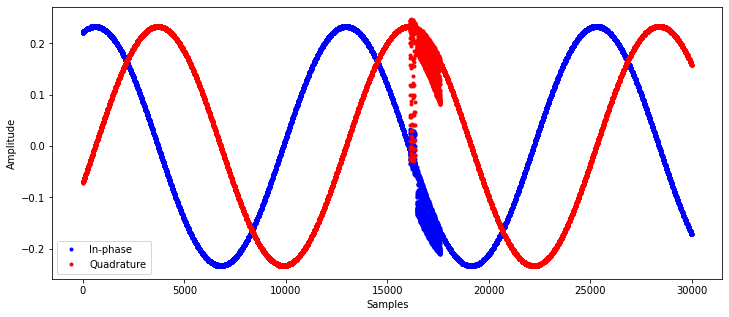
\includegraphics[scale=0.6]{figures/data_IQ-signal.png}
  \caption{In-phase and quadrature signals}
  \label{fig:iq-signal}
\end{figure}

data representation.

% -------------------------------------------------------------------------------------------------------------
\subsection{NFC characteristics}

13.56MHz -- HF

proximity technology

"antenna"

passive tags -- modulation of the reader's field

% -------------------------------------------------------------------------------------------------------------
\subsection{Radio setup}

\begin{figure}[htp!]
  \centering
  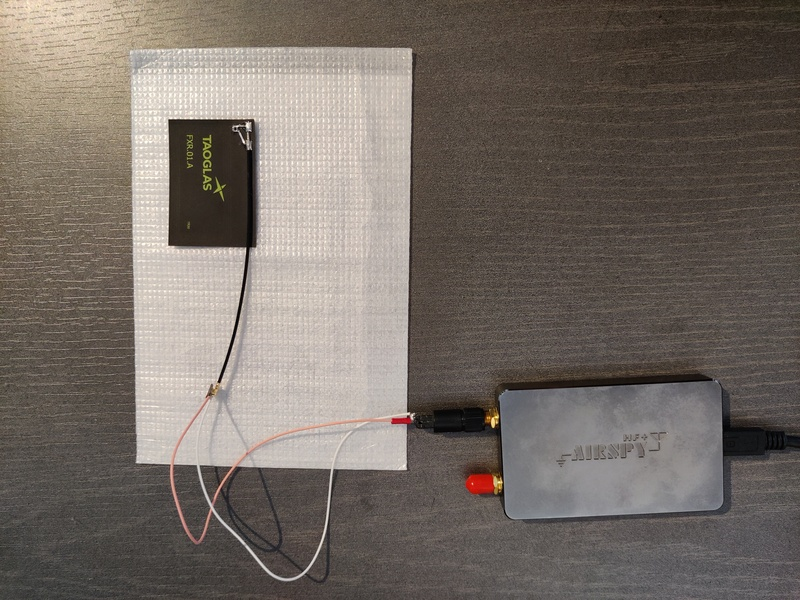
\includegraphics[scale=0.25]{figures/data_sdr-setup2.jpg}
  \caption{SDR and antenna setup}
  \label{fig:radio-setup}
\end{figure}

% -------------------------------------------------------------------------------------------------------------
\subsection{Inventory of devices}

A picture of tags 1 to 7 is provided in figure \ref{fig:tags} and their technical details are listed in table \ref{tab:picc-inventory}. Tags 1 to 5 use the exact same chip...

On tags 1 to 7, the content of the tags is harmonized to ensure the algorithm won't use the content as a feature to identify devices.

\begin{figure}[htp!]
  \centering
  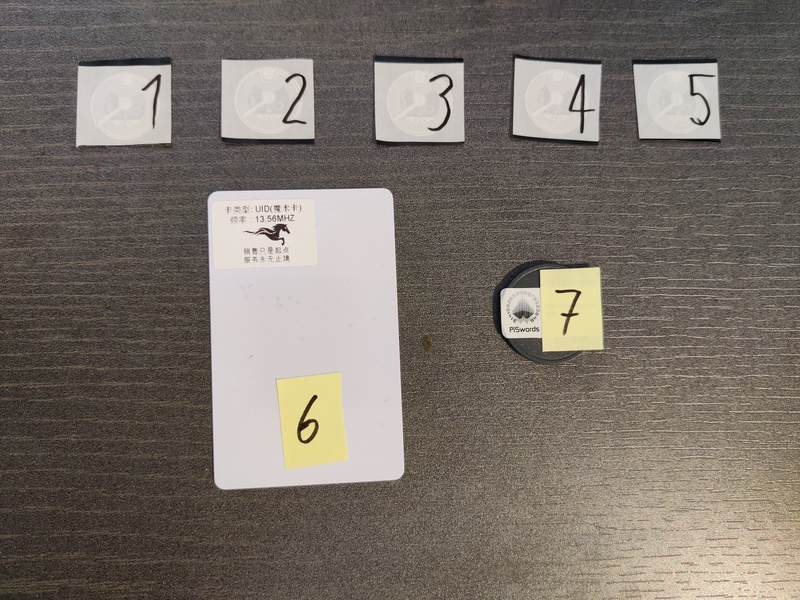
\includegraphics[scale=0.25]{figures/data_standard-tags2.jpg}
  \caption{NFC tags 1-7}
  \label{fig:tags}
\end{figure}

\begin{table}[h!]
  \centering
  \begin{tabular}{|l|l|l|l|l|l|}
    \hline
    \textbf{Name} & \textbf{Standard} & \textbf{NFC type} & \textbf{Chip}     & \textbf{ATQA} & \textbf{SAK} \\ \hline
    \textbf{tag1} & ISO 14443-3A      & NFC-A             & NTAG213           & 0x0044        & 0x00         \\ \hline
    \textbf{tag2} & ISO 14443-3A      & NFC-A             & NTAG213           & 0x0044        & 0x00         \\ \hline
    \textbf{tag3} & ISO 14443-3A      & NFC-A             & NTAG213           & 0x0044        & 0x00         \\ \hline
    \textbf{tag4} & ISO 14443-3A      & NFC-A             & NTAG213           & 0x0044        & 0x00         \\ \hline
    \textbf{tag5} & ISO 14443-3A      & NFC-A             & NTAG213           & 0x0044        & 0x00         \\ \hline \hline
    \textbf{tag6} & ISO 14443-3A      & NFC-A             & Mifare Classic 1k & 0x0004        & 0x08         \\ \hline
    \textbf{tag7} & ISO 14443-3A      & NFC-A             & Mifare Classic 1k & 0x0004        & 0x08         \\ \hline
    \textbf{tag8} & ISO 14443-4       & NFC-A             & Mifare Classic 4k & 0x0002        & 0x38         \\ \hline
    \textbf{tag9} & JIS 6319-4        & FeliCa            & RC-S967           & -             & -            \\ \hline
  \end{tabular}
  \caption{Inventory of PICC devices}
  \label{tab:picc-inventory}
\end{table}

\begin{table}[h!]
  \centering
  \begin{tabular}{|l|l|l|}
    \hline
    \textbf{Name}    & \textbf{Type} & \textbf{Model} \\ \hline
    \textbf{reader1} & Smartphone    & OnePlus 8      \\ \hline
    \textbf{reader2} & Smartphone    & Nexus 6p       \\ \hline
  \end{tabular}
  \caption{Inventory of PCD devices}
  \label{tab:pcd-inventory}
\end{table}

% -------------------------------------------------------------------------------------------------------------
\subsection{Dataset description}

\begin{figure}[htp!]
  \centering
  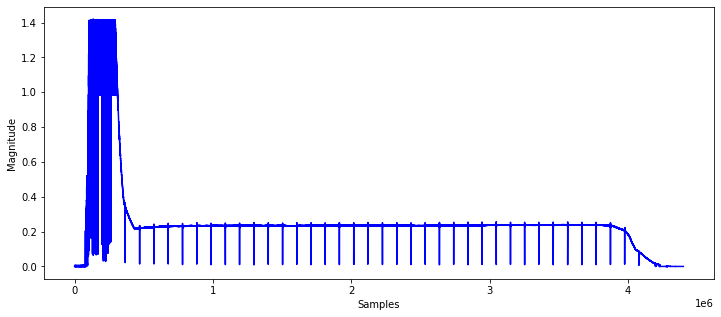
\includegraphics[scale=0.47]{figures/data_whole-transmission.png}
  \caption{Two seconds of NFC communication represented as magnitudes}
  \label{fig:nfc-full}
\end{figure}

\begin{figure}[htp!]
  \centering
  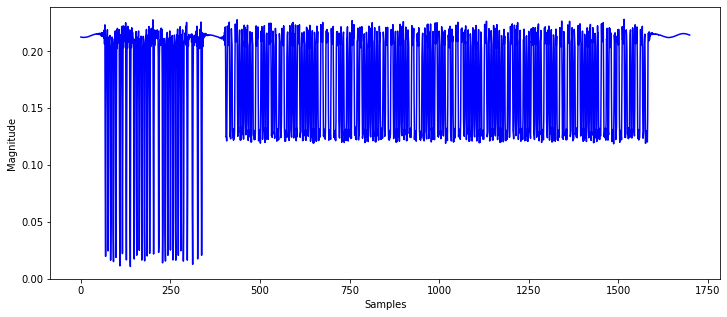
\includegraphics[scale=0.6]{figures/data_single-request-response.png}
  \caption{NFC single request/response represented as magnitudes}
  \label{fig:nfc-single}
\end{figure}

% -------------------------------------------------------------------------------------------------------------
\subsection{Validating the dataset}
